\documentclass[12pt]{article}
\usepackage{KTUstyle}



\begin{document}
% Titulinis puslapis
\begin{titlepage}

\newcommand{\universitetas}{Kauno technologijos universitetas}
\newcommand{\fakultetas}{Informatikos fakultetas}
\newcommand{\katedra}{Kompiuterių katedra}
\newcommand{\pavadinimas}{Skaitmeninės Logikos Pradmenys(P175B100)}
\newcommand{\tipas}{Pirmas Laboratorinis darbas}
\newcommand{\grupe}{IFF 8/11}
\newcommand{\atliko}{Arnas Švenčionis}
\newcommand{\prieme}{dėst. Ignas Pliauska}
\newcommand{\miestas}{Kaunas}
\newcommand{\metai}{\the\year}

\renewcommand{\headrulewidth}{0pt}

    \onehalfspacing
	\center
	
\includegraphics[width=20mm]{ktu} \\
    \LARGE\textbf{\MakeUppercase{\universitetas}} \\ [5mm]
    \Large\textbf{\MakeUppercase{\fakultetas}} \\ [5mm]	
    \large\textbf{\MakeUppercase{\katedra}} \vfill
	{\fontsize{22}{26}\centering\bfseries\MakeUppercase{\pavadinimas}\par} \vfill
    {\centering \Large \tipas} \vfill
    
	\flushright	
	{\center	
		\normalsize
		\begin{tabular}{l}\onehalfspacing	
			\textbf{Atliko:} \\[1.5pt]
			\grupe grupės stud. \\
			\atliko \\[1cm]

			\textbf{Priėmė}\\[1.5pt]
			\prieme
		\end{tabular}
	}
	\vfill
	\center
	\normalsize\textbf{\MakeUppercase{\miestas}, \metai}
\end{titlepage}
		

% Turinys
\tableofcontents

\newpage


\section{Įvadas}

\subsection{Darbo tikslas}


\paragraph{Įsisavinti Būlio funkcijų minimizavimą ir kombinacinių loginių schemų projektavimą bei modeliavimą.}

\subsection{Darbo užduotis}

\paragraph{Užduočių variantų lentelėje duotos funkcijos, kurių argumentų konjunkcijos pateiktos skaičiais. Kiekvienas studentas gauna jam priklausančio varianto numerį. Atlikti užduočiai reikia:}	
\begin{enumerate}
	\item  Užrašyti pateiktą funkciją normaliąja disjunkcine forma;
	\item Minimizuoti pateiktą funkciją;
	\item  Realizuoti šią funkciją trimis būdais: (a) naudojant IR, ARBA, NE elementus, (b) naudojant tik IR-NE arba ARBA-NE ir NE elementus, (c) naudojant multiplekserį ir reikiamus IR, ARBA, NE, IR-NE, ARBA-NE elementus;
	\item Patikrinti suprojektuotų schemų funkcionavimą;
	\item  Paruošti laboratorinio darbo ataskaitą. Ataskaitoje pateikti funkcijos minimizavimo rezultatus, realizuotas schemas bei šių schemų modeliavimo rezultatus.
\end{enumerate}

\paragraph{Mano užduotis:}
3,6,7,11,19,21,24,29,32,34,35,40,41,42,48,49,52,63 

\section{Darbo Atlikimas}

2.1 Užrašome šią funkciją tobula normaliąja disjunkcine forma, sudarome Karno lentelę ir ją užpildome funkcijos reikšmėmis:
	\input{neminimizuota_funkcija.txt}


\begin{table}[!htbp]
	\caption{Karno lentelė.}
	\centering
	\begin{tabular}{|c|c|c|c|c|c|c|c|}
		\hline
		$000$ & $001$ & $011$ & $010$ & $110$ & $111$ & $101$ & $100$ \\
		\hline
		 &  & 1 &  & 1 & 1 &  & \\
		 &  & 1 &  &  &  &  & \\
		1 &  &  &  &  &  & 1 &\\
		 &  & 1 & & &  & 1 &\\
		 1&1&&&&&&1 \\
		 &&&&&1&& \\
		 1&1&&1&&&& \\
		 1&&1&1&&&& \\
		\hline
	\end{tabular}
\end{table}

2.1.1 Pasinaudoję Karno lentele gausime minimizuotą funkcijos išraišką, kurią galima supaprastinti, iškeliant reikiamuosius prieš skliaustus:
	\begin{align}
f &= 
a\bar{b}\bar{d}(c\bar{e}+\bar{e}\bar{f}+\bar{c}e+e\bar{f})
+\bar{a}\bar{d}ef(\bar{b}+\bar{c})
+b\bar{e}(a\bar{c}\bar{d}+\bar{a}df+a\bar{c}\bar{f}+\bar{a}c\bar{d}\bar{f})
+de(\bar{a}\bar{b}\bar{c}+abcf)
\end{align}
	
	\begin{align}
	f &= 
	\overline{\overline{a\bar{b}\bar{d}(\overline{\overline{c\bar{e}}*\overline{\bar{e}\bar{f}}*\overline{\bar{c}e}*\overline{e\bar{f}}})}
	*\overline{\bar{a}\bar{d}ef(\overline{\overline{\bar{b}}*\overline{\bar{c}}})}
	*\overline{b\bar{e}(\overline{\overline{a\bar{c}\bar{d}}*\overline{\bar{a}df}*\overline{a\bar{c}\bar{f}}*\overline{\bar{a}c\bar{d}\bar{f}}})}
	*\overline{de(\overline{\overline{\bar{a}\bar{b}\bar{c}}*\overline{abcf}})}}
\end{align}
	
	\begin{align}
	D_{0} &=
	\bar{a}\bar{d}(\bar{d}ef+\bar{c}ef+bc\bar{e}\bar{f}) \nonumber \\
	&D_{1} &= 
	a\bar{d}(b\bar{c}\bar{e}+\bar{b}c\bar{e}+\bar{b}\bar{e}\bar{f}+\bar{b}\bar{c}e+\bar{b}e\bar{f}) \nonumber \\
	&D_{2} &=
	\bar{a}d(\bar{b}\bar{c}e+b\bar{e}f) \nonumber \\
	&D_{3} &= 
	ad(b\bar{c}\bar{e}\bar{f}+bcef)
\end{align}
	
	\begin{align}
f &=  \bar{a}\bar{b}\bar{c}\bar{d}\bar{e}f+\bar{a}\bar{b}\bar{c}\bar{d}ef+
\bar{a}\bar{b}\bar{c}d\bar{e}\bar{f}+\bar{a}\bar{b}c\bar{d}e\bar{f}+\bar{a}\bar{b}cde\bar{f}\nonumber \\&
+\bar{a}bcde\bar{f}+\bar{a}b\bar{c}\bar{d}\bar{e}\bar{f}+\bar{a}b\bar{c}de\bar{f}+\bar{a}b\bar{c}def+ab\bar{c}\bar{d}\bar{e}\bar{f}\nonumber \\&
+ab\bar{c}\bar{d}e\bar{f}+ab\bar{c}de\bar{f}+ab\bar{c}d\bar{e}f+ab\bar{c}d\bar{e}\bar{f} +abc\bar{d}\bar{e}f\nonumber \\&
+a\bar{b}c\bar{d}e\bar{f}+a\bar{b}\bar{c}\bar{d}\bar{e}\bar{f}+a\bar{b}\bar{c}b\bar{e}\bar{f}
\label{eq:1}
\end{align}

\begin{align}

C &= {x}_{1}\nonumber \\&
\bar{R} &= ({x}_{2}\cup{x}_{3})\oplus{x}_{4}\nonumber \\&
S &= ({x}_{2}\cup{x}_{3})*\bar{x}_{4}
\end{align}
	

\subsection{Formulės} \label{formules}
\eqref{eq:2} pateikta vienos eilutės formulė, \eqref{eq:1} -- dviejų eilučių formulė.

\subsubsection{Vienos eilutės formulė} \label{vienos}
\begin{equation}
	f = \bar{x}_{1}\bar{x}_{2}\bar{x}_{3}\bar{x}_{4}\bar{x}_{5}\bar{x}_{6}\cup x_{1}\bar{x}_{2} x_{3} x_{4} x_{5}\bar{x}_{6}. \label{eq:2}
\end{equation}

\subsubsection{Kelių eilučių formulė} \label{keliu}
    \input{neminimizuota_funkcija.txt}  
 

 
\subsection{Lentelės} \label{lenteles}

\begin{table}[!htbp]
\caption{Funkcijos teisingumo lentelė.}
	\centering
	\begin{tabular}{|cc|c|}
		\hline
		$x_1$ & $x_2$ & $y$ \\
		\hline
		0 & 0 & 1 \\
		0 & 1 & 0 \\
		1 & 0 & 0 \\
		1 & 1 & 1 \\
		\hline
	\end{tabular}
\end{table}


\subsection{Paveikslai} \label{paveikslai}

\ref{fig:11} pav. pavaizduotas pirmasis namas, \ref{fig:12} pav. -- antrasis namas. \ref{fig:2} pav. pirmasis namas pavaizduotas didesniu formatu. 

\begin{figure}[!htbp] 
\centering
\subfloat[Pirmas namas]{\label{fig:11}%
  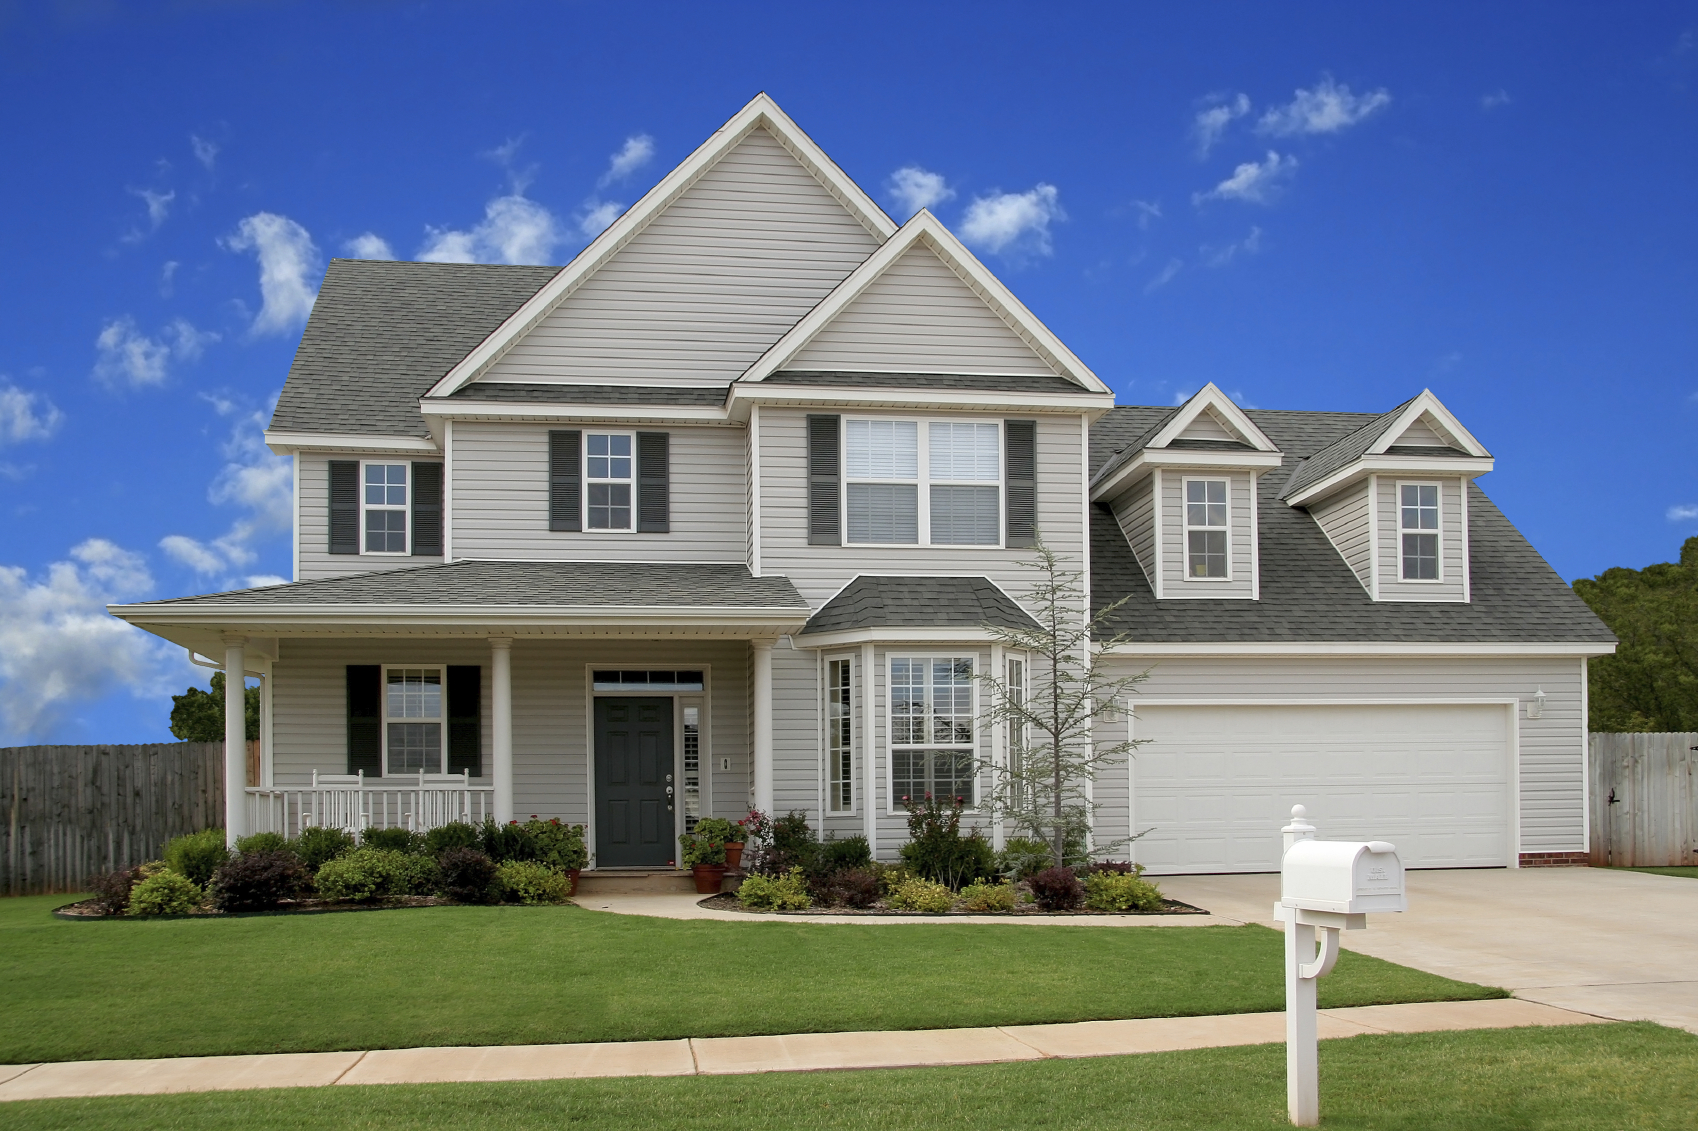
\includegraphics[height=5cm]{house1}}\ %
\subfloat[Antras namas]{\label{fig:12}%
  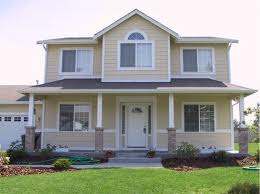
\includegraphics[height=5cm]{house2}}
\caption{Pirmas ir antras namai.}
\label{fig:1} 
\end{figure} 

\begin{figure}[!htbp]
\centering
	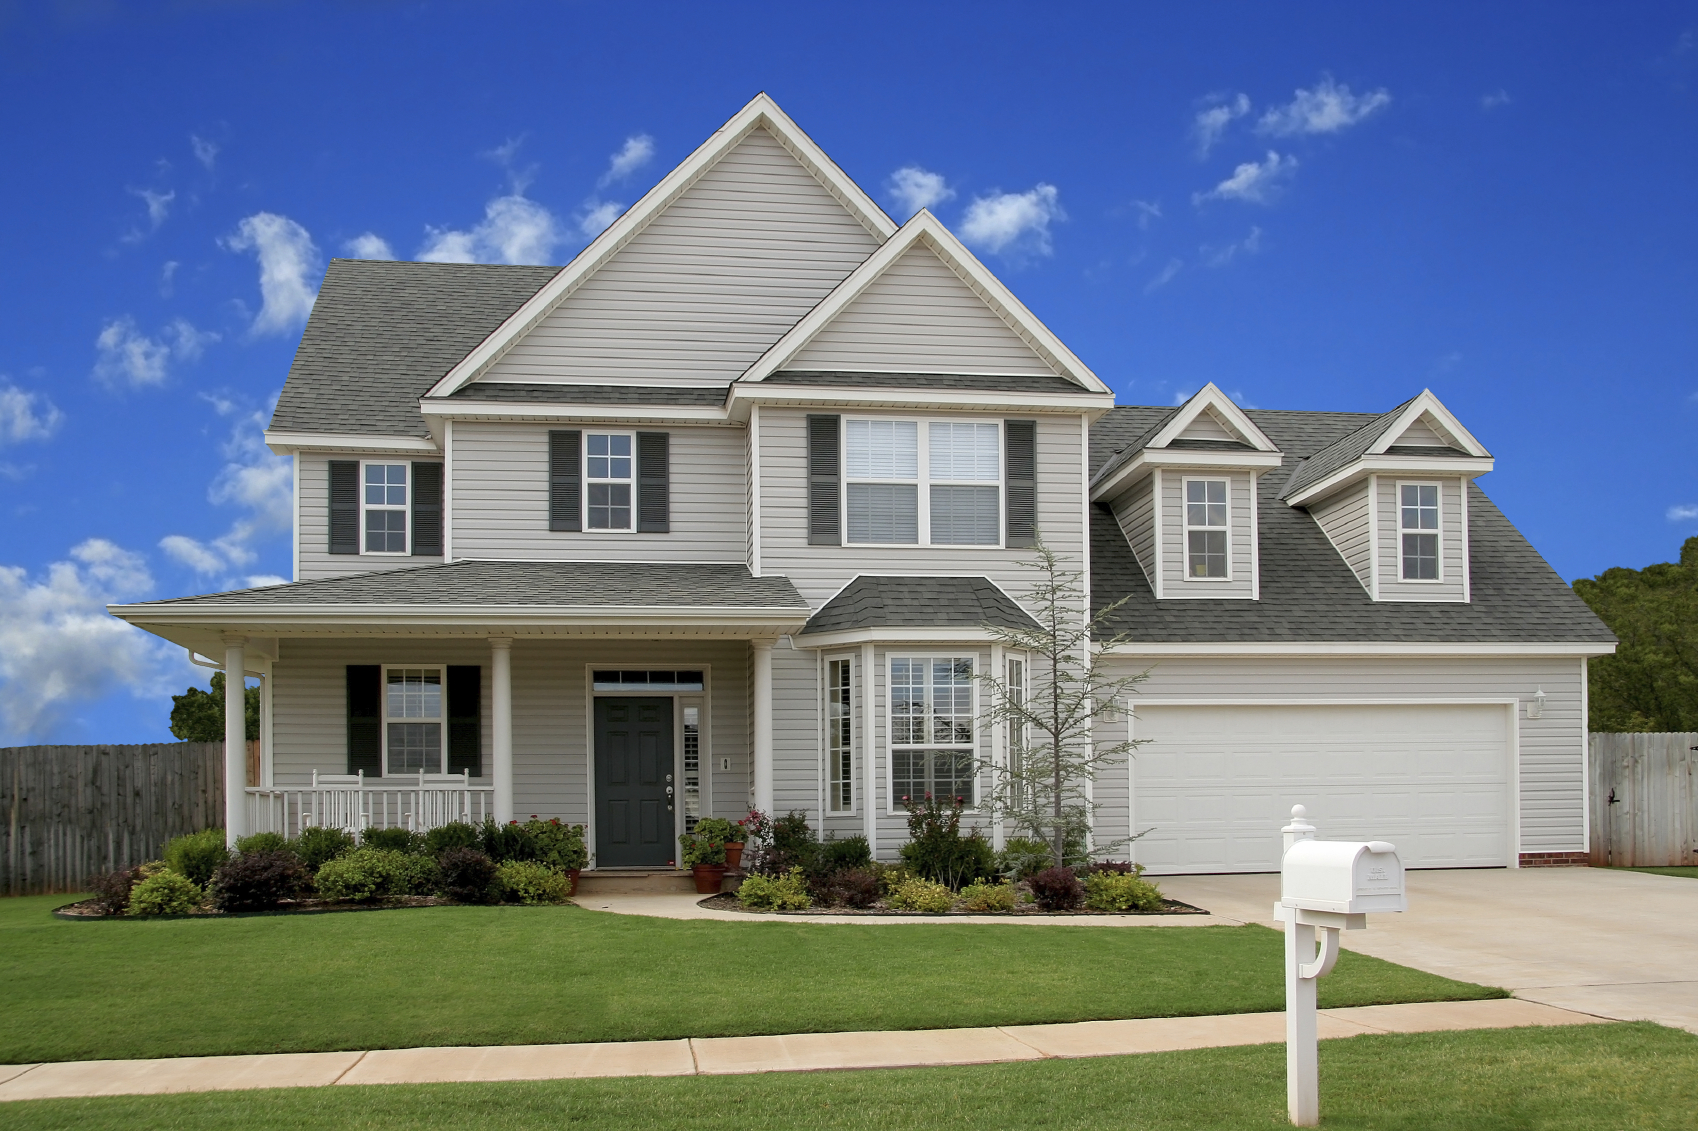
\includegraphics[height=8cm]{house1}
	\caption{Didelis pirmas namas.}
	\label{fig:2}
\end{figure}

\ref{fig:2} pav. namą galima rasti \cite{namas} šaltinyje.

\newpage
% Literaturos sarasas
\newpage

\bibliographystyle{plain}  
\begin{thebibliography}{99}

\phantomsection
\addcontentsline{toc}{section}{Literatūra}\label{literatura}


\bibitem{meng}
Meng X. Implantable Wireless Devices for the Monitoring of Intracranial 
Pressure // X. Meng, U. Kawoos, S. M. Huang, M. R. Tofighi // IEEE 16th International Symposium. -- 2012.


\bibitem{north}
North B. Intracranial pressure monitoring //P. Reilly, R. Bullock. Head Injury; Chapman \& Hall, London, 1997.

\bibitem{popovic}
Popovic D. Noninvasive Monitoring of Intracranial Pressure / D. Popovic, M. Khoo, S. Lee // Recent Patents on Biomedical Engineering. -- 2009, 2, p. 165-179.

\bibitem{namas} 
\url{http://streetinfo.com/6-tips-hosting-great-open-house/}

\end{thebibliography}

\end{document}

